\vspace{0.25cm}\\
\begin{minipage}{0.49\textwidth}
    \centering
    \vspace{0.1cm}
    \begin{figure}[H]
    \centering
    \begin{tikzpicture}[level distance=1.5cm,
        level 1/.style={sibling distance=3cm},
        level 2/.style={sibling distance=1.5cm},
        every node/.style = {minimum width = 2em, draw, circle}
        ]
        \node {5}
            child {node[fill=blue!70] {\textbf{3}}
                child {node {1}}
                child {node[fill=!10!orange] {4}}
            }
            child {node {6}
                child {edge from parent[draw = none]}
                child {node {8}}
            };
    \end{tikzpicture}
    \caption{Find the node you want to remove (orange), in this case the one with  value 4, and that node's parent (blue)}
    \label{fig:nodeleaf}
    \end{figure}
\end{minipage}
\hfill
\begin{minipage}{0.49\textwidth}
    \centering
    \begin{figure}[H]
    \centering
    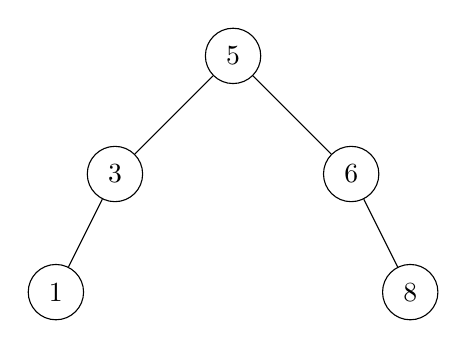
\begin{tikzpicture}[level distance=1.5cm,
        level 1/.style={sibling distance=3cm},
        level 2/.style={sibling distance=1.5cm},
        every node/.style = {minimum width = 2em, draw, circle}
        ]
        \node {5}
            child {node {3}
                child {node {1}}
                child {edge from parent[draw = none]}
            }
            child {node {6}
                child {edge from parent[draw = none]}
                child {node {8}}
            };
    \end{tikzpicture}
    \caption{Set the parent's reference to that node, in this case \lstinline|parent.left| equal to \lstinline|null| to remove the node}
    \label{fig:nodeonechild}
    \end{figure}
\end{minipage}\\
\vspace{0.25cm}\\
The removal of a leaf is perhaps the most straightforward operation. In the
event that both the right and the left points of a node are null then we only
need remove the reference from that node's parent to it.



